\begin{figure*}[t!]
\centering
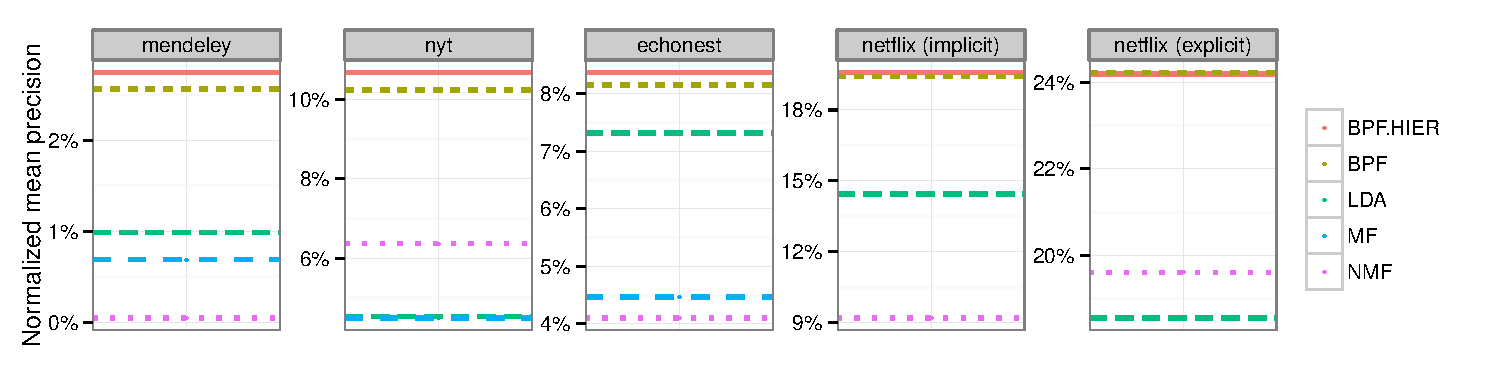
\includegraphics[width=\textwidth]{figures/mean_precision_at_20.pdf}\\
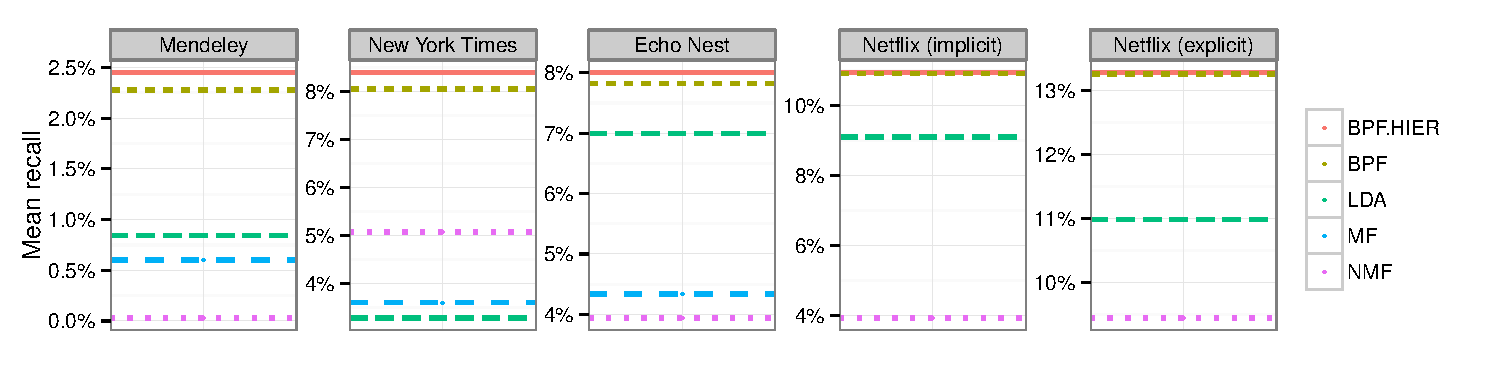
\includegraphics[width=\textwidth]{figures/mean_recall_at_20.pdf}\\
\caption{Predictive performance on data sets. The top and bottom plots
  show normalized mean precision and mean recall at 20
  recommendations, respectively. While baseline performance varies
  across data sets, HPF and BPF consistently outperform competing
  methods.}
\label{fig:precision_recall}
\end{figure*}


\section{Empirical Study}
\label{sec:eval}
We evaluate the performance of the Hierarchical Poisson factorization
(HPF) algorithm and its non-hierarchical variant (BPF) on a variety of
large-scale data sets for the purpose of recommending new items to
users. We first discuss details of each data set and of competing
recommendation methods. In particular, we note the superior
performance and computational efficiency of Poisson factorization in
comparison to baseline methods. We conclude with an exploratory
analysis of the preferences and attributes inferred by HPF.

{\bf Data Sets.} We study the HPF algorithm in Figure~\ref{fig:batch}
on several data sets of user behavior that contain both implicit
and explicit feedback:
\begin{itemize}
\item The {\bf Mendeley} data set~\cite{Jack:2010} of scientific
  articles is a binary matrix of 80,000 users and 260,000 articles,
  where each of the 5 million observations corresponds to the presence
  of an article in a user's online library.
\item The {\bf Echo Nest} music data set~\cite{Bertin-Mahieux:2011}
  consists of 1 million users, 385,000 distinct songs and 48 million
  (user, song, play count) triplets.
\item The {\bf New York Times} data set with 1,615,675 users, 103,390
  articles, and 80 million (user, article, view count)
  observations.
\item The {\bf Netflix} data set~\cite{Koren:2009} consists of 480,000
  users, 17,770 movies and 100 million ratings, where each observation
  is an explicit rating (from 1 to 5 stars) that a user provided for
  the given movie.
  discarded~\cite{Paquet:2013p9197}.
\end{itemize}

The scale and diversity of these data sets enables a robust evaluation
of our algorithm. The Mendeley, Echo Nest, and New York Times data
sets are sparse in comparison to the movie data. For example, we
observe only 0.001\% of all possible user-item ratings in Mendeley,
while 1\% of the ratings are non-zero in the Netflix data. This is
partially a reflection of large number of items relative to number
users in these data sets.

Furthermore, the intent signaled by an observed rating varies
significantly across these data sets. For instance, the Netflix data
set gives the most direct measure of stated preferences for items, as
users provide an explicit star rating for movies they have watched. In
contrast, article click counts in the New York Times data are a less
clear measure of how much a user likes a given article---most articles
are read only once, and a click through is only a weak indicator of
whether the article was fully read, let alone liked. Ratings in the
Echo Nest data presumably fall somewhere in between, as the number of
times a user listens to a song likely reveals some indirect
information about their preferences.

As such, we treat each data set as a source of implicit feedback,
where an observed positive rating indicates that a user likes a
particular item, but the rating value itself is ignored. The Mendeley
data are already of this simple binary form. For the Echo Nest and New
York Times data, we consider any song play or article click as a
positive rating, regardless of the play or click count. We also
consider two versions of the Netflix data---the original, explicit
ratings, and an implicit version in which only 4 and 5 star ratings
are retained as observations~\cite{Paquet:2013p9197}.


{\bf Baselines.} We compare Poisson factorization against an array of
competing methods:
\begin{itemize}
  \item {\bf NMF}: Non-negative Matrix
    Factorization~\cite{Lee:1999}. In NMF, user preferences and item
    attributes are modeled as non-negative vectors in a
    low-dimensional space. These latent vectors are randomly
    initialized and modified via an alternating multiplicative update
    rule to minimize the Kullback-Leibler divergence between the
    actual and modeled rating matrices.

  \item {\bf LDA}: Latent Dirichlet Allocation~\cite{Blei:2003b}. LDA
    is a Bayesian probabilistic generative model where user preferences
    are represented by a distribution over different topics, and each
    topic is a distribution over items. Interest and topic
    distributions are randomly initialized and updated using
    stochastic variational inference~\cite{Hoffman:2010a} to
    approximate these intractable posteriors.

  \item {\bf MF}: Matrix Factorization with user and item biases. We
    use a variant of matrix factorization popularized through the
    Netflix Prize~\cite{Koren:2009}, where a linear
    predictor---comprised of a constant term, user activity and item
    popularity biases, and a low-rank interaction term---is fit to
    minimize the mean squared error between the predicted and observed
    rating values, subject to L2 regularization to avoid
    overfitting. Weights are randomly initialized and updated via
    stochastic gradient descent using the Vowpal Wabbit
    package~\cite{Weinberger:2009}. This corresponds to maximum
    a-posteriori inference for a Gaussian likelihood model.

\end{itemize}

We note that while HPF, BPF, and LDA take only the non-zero observed
ratings as input, traditional matrix factorization requires that we
provide explicit zeros in the ratings matrix as negative examples,
even in the implicit feedback setting. In practice, this amounts to
either treating all missing ratings as zeros (as in NMF) and
down-weighting to balance the relative importance of observed and
missing ratings~\cite{Hu:2008p9402}, or generating negatives by
randomly sampling from missing ratings in the training
set~\cite{Dror:2012a}.

We take the latter approach for computational convenience, employing a
popularity-based sampling scheme: we sample users by activity---the
number of items rated in the training set---and items by
popularity---the number of training ratings an item received to
generate negative examples.\footnote{We also compared this to a
  uniform random sampling of negative examples, but found that the
  popularity-based sampling performed better.} We note that this
procedure is relatively expensive for large-scale data sets, and
results in scaling difficulties for methods such as Bayesian
Personalized Ranking (BPR)~\cite{Rendle:2009p9243,Gantner:2012p9364},
which iteratively perform such sampling over dozens of iterations. In
particular, we found this to be prohibitive when attempting to use BPR
with the data sets considered here.

%% attempted to get SIGIR code, but failed

\begin{figure*}[t!]
\centering
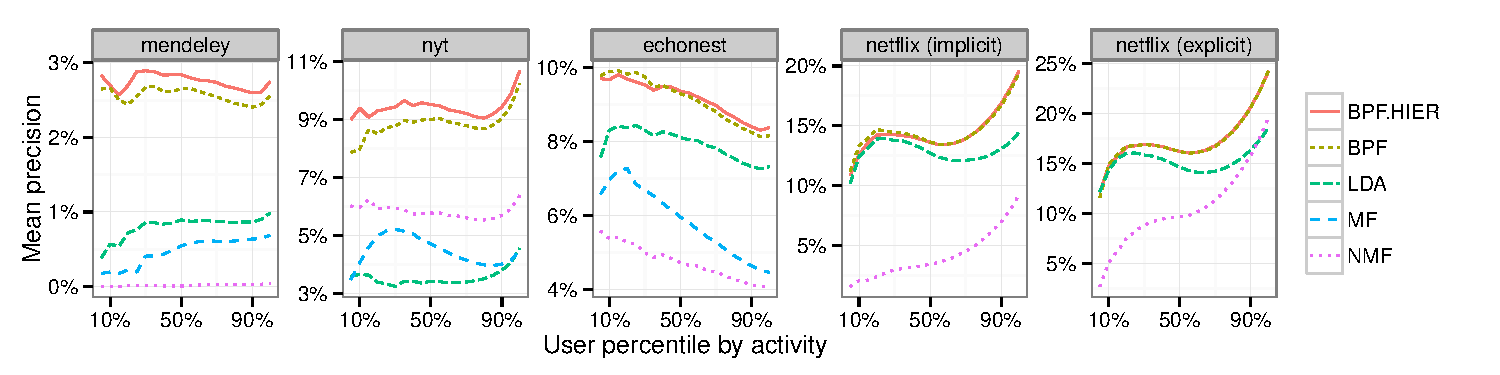
\includegraphics[width=\textwidth]{figures/mean_precision_at_20_by_user_percentile.pdf}\\
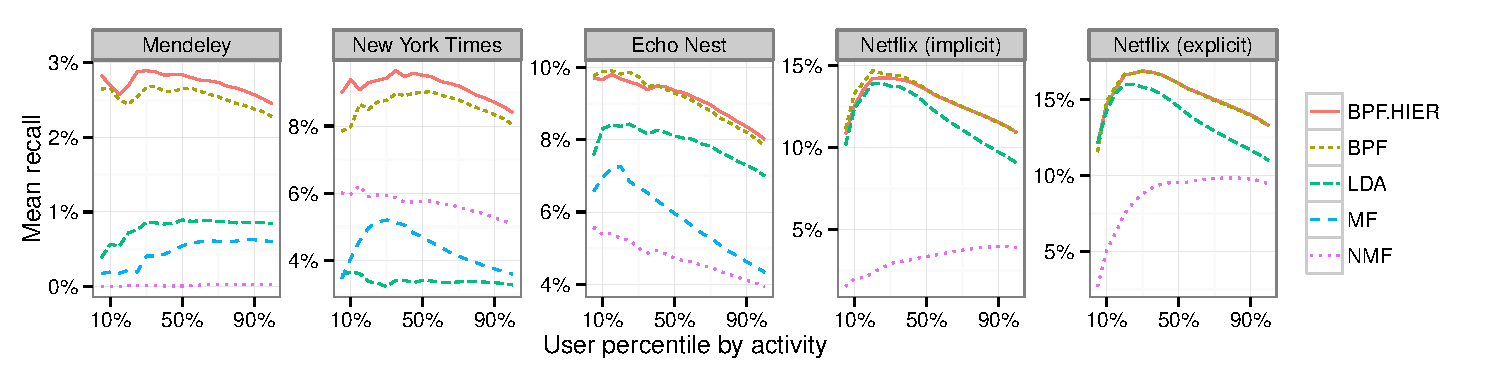
\includegraphics[width=\textwidth]{figures/mean_recall_at_20_by_user_percentile.pdf}\\
\caption{Predictive performance across users. The top and bottom plots
  show normalized mean precision and mean recall at 20
  recommendations, respectively, by user activity.}
\label{fig:precision_recall_by_user_activity}
\end{figure*}

{\bf Evaluation.} Prior to training any models, we randomly select
20\% of ratings in each data set to be used as a held-out test set
comprised of items that the user has consumed. Additionally, we set
aside 1\% of the training ratings as a validation set and use it to
determine algorithm convergence and to tune free parameters. For HPF
and BPF we find that the algorithm is largely insensitive to small
changes in the hyper-parameters.

During testing, we generate the top $M$ recommendations for each user
as those items with the highest predictive score under each
method. For each user, we compute a variant of precision-at-$M$, which
measures the fraction of relevant items in the user's top-$M$
recommendations. So as not to artificially deflate this measurement
for lightly active users who have consumed fewer than $M$ items, we
compute {\it normalized} precision-at-$M$, which adjusts the
denominator to be at most the number of items that the user has in the
test set. Likewise, we compute recall-at-$M$, which captures the
fraction of items in the test set present in the top $M$
recommendations.

%% \begin{equation*}
%%   \textrm{NPrec}@M = \frac{|~\textrm{relevant items at $M$ recommendations}~|}
%%          {\mathrm{min}(M, |~\textrm{relevant items}~|)}
%% \end{equation*}

\myfig{precision_recall} shows the normalized mean precision at 20
recommendations for each method and data sets. We see that HPF and BPF
outperform other methods on all data sets by a sizeable margin---as
much as 8 percentage points. Likewise, Poisson factorization shows
similar gains in recall over traditional MF approaches, indicated in
\myfig{recall_by_M}---a relatively high fraction of items recommended
by HPF are found to be relevant, and many relevant items are
recommended. While not shown in these plots, the relative performance
of methods within a data set is consistent as we vary the number of
recommendations shown to users. We also note that while Poisson
factorization dominates across all of these data sets, the relative
quality of recommendations from baseline methods varies substantially
from one dataset to the next. For instance, LDA performs quite well on
the Echo Nest data, but fails to beat classical matrix factorization
for the implicit Netflix data set.

We also study precision as a function of user activity to investigate
how performance varies across users of different types. In particular,
\myfig{precision_recall_by_user_activity} shows the mean normalized
precision and mean recall at 20 recommendations as we look at
performance for users of varying activity, measured by
percentile. (For example, the 10\% mark shows mean performance across
the bottom 10\% of users, who are least active; the 90\% mark shows
the mean performance for all but the 10\% of most active users.) Here
we see that Poisson factorization outperforms other methods for users
of all activity levels---both the ``light'' users who constitute the
majority, and the relatively few ``heavy'' users who consume
more---for all data sets. For the New York Times and Netflix data, we
see that higher levels of user activity enable us to better estimate
user preferences and improve the quality of recommendations. For the
Mendeley and Echo Nest data, however, we see a decline in normalized
precision for the heavy users. Presumably this difference is due to
the large catalogues of items relative to the number of users in these
data sets, comparatively. We also note that the decrease in mean
recall as we consider increasingly active sets of users is inevitable,
as these individuals have a larger set of relevant items in the test
set than their less active counterparts.

{\bf Exploratory analysis.} The fitted model can be explored to
discover latent structure among items and users and to confirm that
the model is capturing the components in the data in a reasonable
way. For example, in \myfig{components} we illustrate the components
discovered by our algorithm on the scientific articles in Mendeley,
movies in Neflix and articles in the New York Times. For each data
set, the illustration shows the top 10 items---items sorted in
decreasing order of their expected weight $\beta_i$---from three of
the 100 components discovered by our algorithm. These components
naturally organize the movies and articles, and enable recommendation
of new items to the user.

In \myfig{movielens-illustration} we show a subset of the highly rated
movies of a user from the MovieLens data
set~\cite{Herlocker:1999}. The top 15 movies recommended to this user
using the trained HPF model, are also shown. The user's ratings are
for primarily drama movies. We movies HPF recommends closely resemble
the types of drama movies she is interested in, for example,
``Children's drama'' or ``War drama''. The expected user's $K$-vector
of weights $\theta_u$, inferred by our algorithm, is shown in
\myfig{movielens-illustration}. In our analysis, $K$ was set to
100. The $\theta_u$ are not sparse because the user's views span a
range of movies in the small data set.

\begin{figure*}
\centering
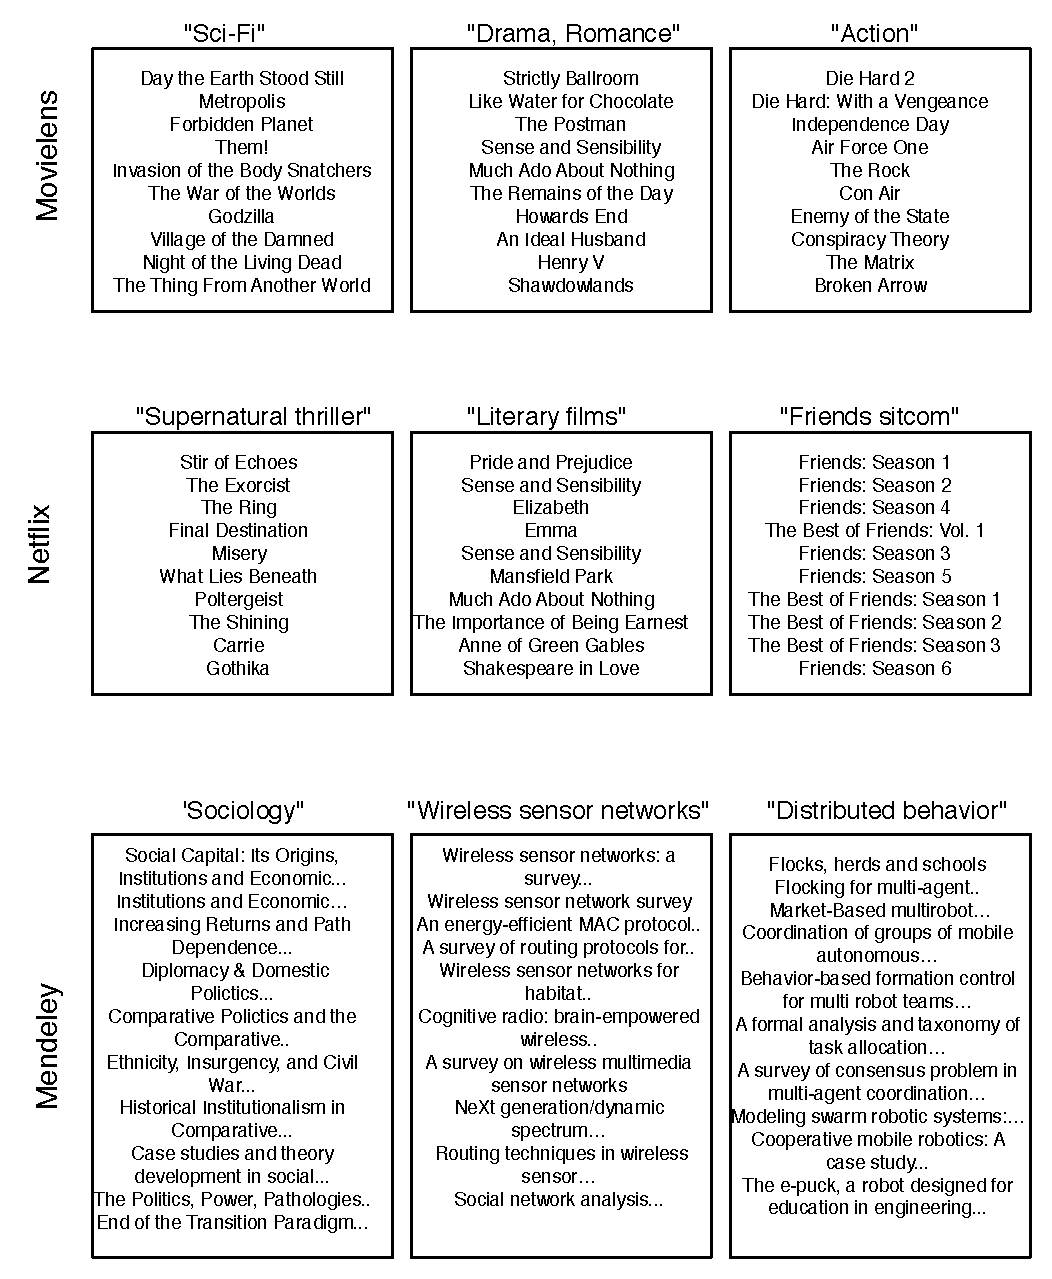
\includegraphics[width=\textwidth]{./figures/components.pdf}
\caption{The top 10 items by the expected weight $\beta_i$ from three
  of the 100 components discovered by our algorithm.}
\label{fig:components}
\end{figure*}
